 \documentclass[a4paper]{article}

\usepackage[english]{babel}
\usepackage[utf8x]{inputenc}
\usepackage{amsmath}
\usepackage{graphicx}
\usepackage[colorinlistoftodos]{todonotes}
\usepackage[margin=1in]{geometry}
\setlength{\parindent}{0pt}
\usepackage{url}
\usepackage{float}
\usepackage[section]{placeins}
 

\title{Mathematical and Data Modelling 2 \\ Ley Lines}

\author{Phoebe Alden, Jack Crago, Ben Goss and Ben Willsher}

\date{\today}

\begin{document}

\pagenumbering{gobble}

\maketitle

\pagebreak

\begin{abstract}
\noindent
The question in hand was to investigate a set of sites built during the Neolithic period across Britain and Ireland. A particular point to be studied was whether any lines stretching between a number of sites (Ley Lines), could be found to be statistically significant. Any other notable patterns within the data were to be investigated as well.
\newline\newline
The Hough transform was used to search for lines between all of the locations in the dataset, allowing for a 50m tolerance on either side of the line, and the most densely populated Ley Line was found to contain seven points. The transform was then used one thousand times on random data, and it was found that in one hundred and forty four cases the most densely populated line found had seven or more sites within the tolerance. This meant that the line was discarded as statistically insignificant.
\newline\newline
The DBSCAN clustering algorithm was also used to find clusters in the Neolithic sites. Eight significant clusters were found. The algorithm was also used to find clusters in one thousand random datasets, not finding a single significant cluster. This was taken to mean that clusters of the size and density as those found within the Neolithic sites are statistically significant.
\newline\newline
From this it was concluded that while Ley Lines do not exist, and did not contribute to line of sight navigation, large and dense clusters were notable within the data, suggesting that there were large communities of Neolithic people who lived in these areas thousands of years ago.
\end{abstract}

\clearpage

\tableofcontents

\clearpage

\pagenumbering{arabic}

\section{Introduction}
The idea of Ley Lines was created when the amateur archaeologist Alfred Watkins stopped his car to look at a Roman camp being excavated in Herefordshire. He claims that as he stood there he "saw" straight lines stretching out across the country. Watkins believed that the due to the lack of roads before the Roman settlement in Britain, a form of navigation was needed for the Britons. He believed that beginning in the Neolithic times a system of navigation by line of sight had existed, with monuments as the markers \cite{Alfred Watkins}.
\newline\newline
In 1969 the new age movement, who linked Alfred Watkins’ theory with that of Feng Shui, revived the Ley Lines theory. It is this that has led to the mystical connotations of Ley Lines, and led to the theory being branded a pseudo-science.
\newline\newline
Given a dataset as large as the one containing the locations of all the known sites from the Neolithic Period (4500-2000BC) across the United Kingdom, finding some lines running through multiple points is to be expected. Therefore it was important to calculate whether any lines found throughout the project run through enough sites to be statistically relevant.
\newline\newline
The question in hand was to analyse a data set containing the locations of Neolithic sites across the United Kingdom, and search for any notable lines running through the sites, and also investigate any other statistically notable patterns or shapes that are displayed within the dataset. 

\section{The Data}
Initially, the locations of 1438 Neolithic sites across the British Isles were provided along with a set of 160,754 data points outlining the coastline of the British Isles. To test the significance of any patterns found in the Neolithic sites a method of generating random data points, within the border of the British Isles, had to be produced. To do this, new coastline data was found which provided the information necessary to create the random data points.

\subsection{Coastline Data Points: Old and New}
The initial coastline data, containing the locations of points along the coastline of the British Isles, created a good space to plot the locations Neolithic sites, as can be seen in Figure \ref{fig:ocl}. This enabled their position in the country to be seen, allowing the investigation, and possible explanation, of any patterns found.

\begin{figure}[H]
\centering
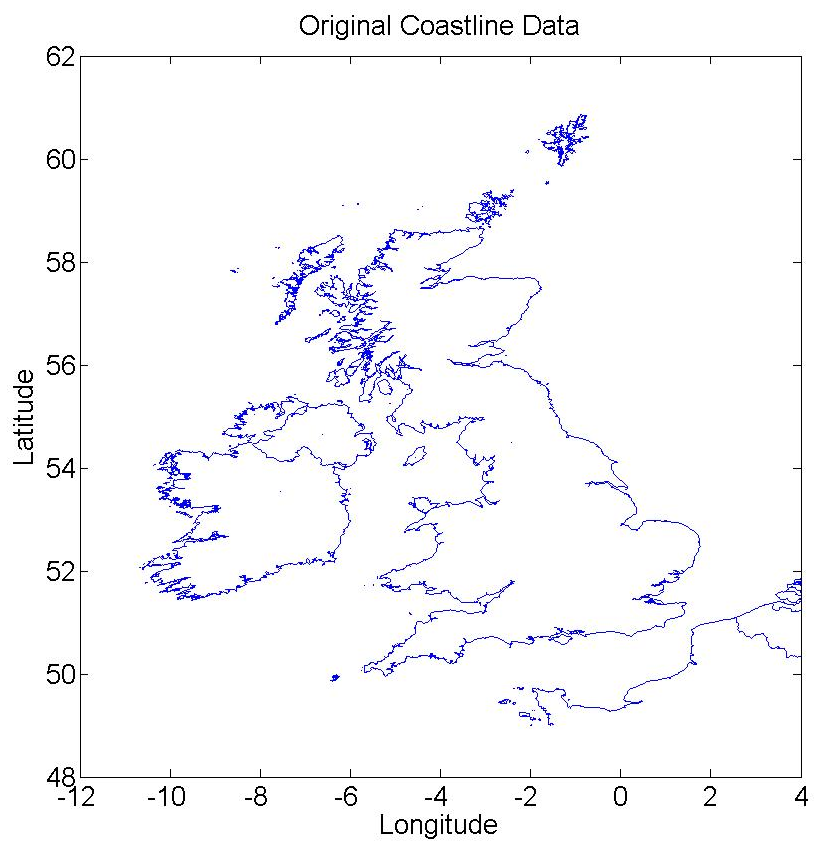
\includegraphics[width=0.4\textwidth]{OCLv2.png}
\caption{\label{fig:ocl}A Graph showing the plot of the Brisish Isles using the original 160,754 coastine data points.}
\end{figure}

While the coastline data was sufficient for the plotting of the locations of the Neolithic sites and looking for patterns, it was problematic when it came to creating a set of inland random data points. To overcome this another set of data, provided by Global Administrative Areas \cite{GAA}  was used. This not only provided higher quality data, as seen in Figure \ref{fig:ncl}, but it also stored the data in polygons which made confining random points within the British Isles much simpler. 

\begin{figure}[H]
\centering
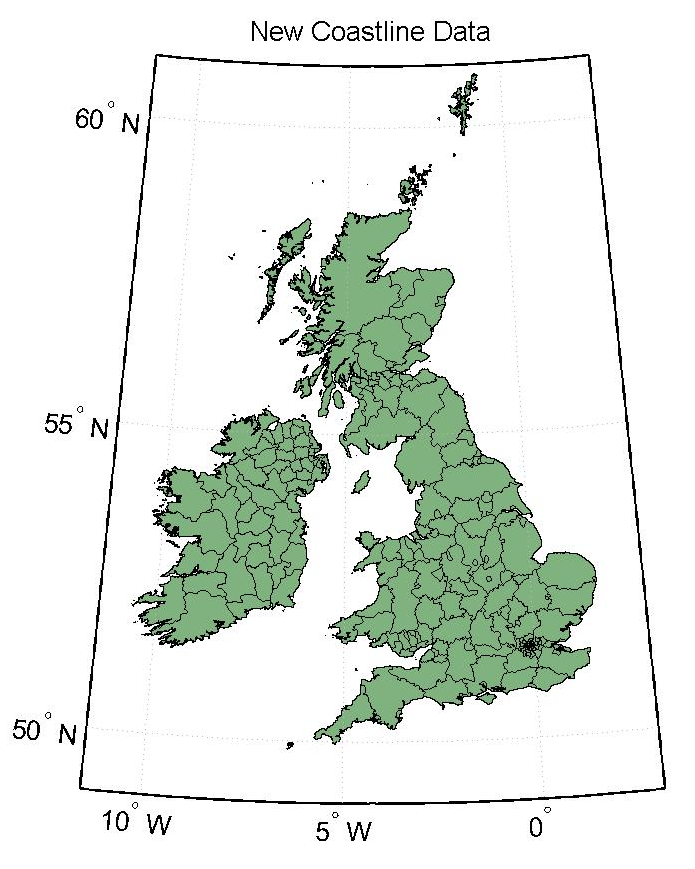
\includegraphics[width=0.35\textwidth]{NCL.png}
\caption{\label{fig:ncl}A Graph showing the plot of the new, higher quality coastline ploygon data.}
\end{figure}

\subsection{1438 Neolithic Sites in the British Isles}
The red points seen in Figure \ref{fig:NSBI} show the locations of Neolithic sites in the British Isles. It can easily be seen that there are more densely concentrated areas of Neolithic sites and some areas which have very few. This is particularly notable in the South East of England. It was theorised that this is due to the fact that the South East is now more highly populated than other parts of the country, and therefore Neolithic sites which did exist have since been built over and lost. 

\begin{figure}[H]
\centering
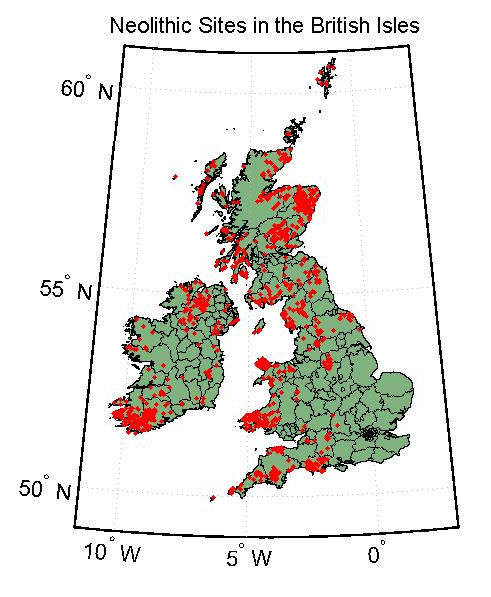
\includegraphics[width=0.35\textwidth]{NSBI.png}
\caption{\label{fig:NSBI}A graph showing the locations of all 1438 Neolithic Sites in the British Isles. It clearly shows that there are a much higher concentration of points in some area than others.}
\end{figure}

\subsection{Creating the Random Sites}
Any patterns found in the Neolithic sites had to be tested to see whether they were statistically significant. To do this, a set of random sites the same size as the matrix of Neolithic sites, was produced. Then, the same pattern analysis that was applied to the Neolithic sites was applied to the random sites. If patterns similar to those found in the Neolithic sites appear regularly in the random sites, then it can be said that the patterns are not statistically significant. However, if the patterns rarely appear in the random sites, then it can be assumed that they are statistically significant and therefore there must be a reason why the patterns found exist. 
\newline \newline
Creating the random sites was problematic due to the unique boundary created by the coastline of the British Isles. Initially the random sites were created within a square boundary around the British Isles, as shown in Figure \ref{fig:RSSB}. 

\begin{figure}[H]
\centering
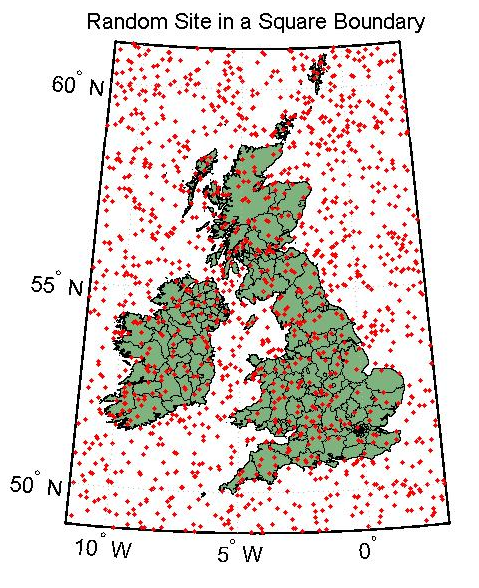
\includegraphics[width=0.35\textwidth]{RSSBv2.png}
\caption{\label{fig:RSSB}A graph showing 1438 random site not confined to the boundary of the British Isles. There are a significant number of sites at sea which is unsatisfactory.}
\end{figure}

The locations of the sites in Figure \ref{fig:RSSB} are highly unrealistic since a significant number of them are in the sea. To find a more realistic representation, the sites that lay outside of the coastlines (in the sea) were removed; this was made possible with the new coastline data. A new set of random sites was created to replace the points which had been removed. This process was repeated until there was a full set of random sites within the coastline boundary, as shown in Figure \ref{fig:RSC}.

\begin{figure}[H]
\centering
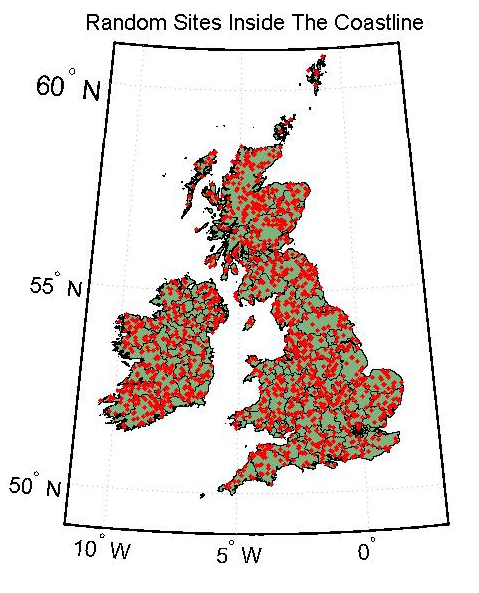
\includegraphics[width=0.35\textwidth]{RSC.png}
\caption{\label{fig:RSC}A graph showing 1438 random site confined to the boundary of the British Isles.}
\end{figure}

\section{Searching for Ley Lines in the Neolithic Sites}
Before attempting to find any lines in the data it was first necessary to decide what the maximum distance between a point and a line is for it to be considered significant. It was decided that a tolerance of 50m was acceptable either side of a line.

\subsection{First Algorithm}
The first attempt to find Ley Lines used a simple algorithm to create lines between data points. The algorithm began by sorting the points, based on their x value, in ascending order. It then created a line joining the first point to the third point in the sorted list, the Euclidean distance between the second point and this line was calculated and compared to the tolerance. The number of points inside the tolerance was recorded and the steps repeated, this time creating a line between the first point and the fourth point, and calculating the distance to all points between the start point and the end point, in this case the second and third. This continued until a line between the first point and all other points had been created and checked. 
\newline\newline
The algorithm then repeated these steps using the second point as the start of the lines and the fourth point up to the last as the ends. This continued up to the antepenultimate point, which created a line with the last point and the distance to the penultimate point was calculated. 
\newline\newline
This is a valid algorithm as it will find a solution and terminate in a finite time, however it is too slow when processing large data sets as the complexity of the algorithm is O($n^3$) . Since this algorithm was not sufficient to solve the problem an alternative way to find lines in the data set was required. To do this the Hough transform was used, this is a global method for finding straight lines hidden in larger amounts of other data \cite{Hough Transform}. It is a much faster algorithm that is better suited to a large data set. 
 
\subsection{Hough Transform}
To use the Hough transform the data had to be interpreted in a different way. Given that the general equation of a straight line is y = mx+c, where m is the gradient and c is the y-intercept, the equation can be rearranged to give c = -mx + y \cite{Hough Transform 2}. For a fixed point [x,y]  the value of m can be varied to create a series of straight lines with varying intercept and gradient, this (m,c) space is called the Hough space. Each point in the Hough space relates to a line in the (x,y) space, and a line in the Hough space represents all straight lines through a fixed point in the (x,y) space. If two points are on a line in the (x,y) space their lines in the Hough space will intersect, so multiple points on a line in the (x,y) space will be a series of lines intersecting at a point in the Hough space. 
\newline\newline
Although this works well it has one major drawback: a vertical line is represented as x=a, if the original equation of a line is used the gradient, m, is undefined. To avoid this an alternative system is used where a line is represented using two variables r and $\theta$, where r is the distance from the origin to the line along a vector perpendicular to the line and $\theta$ is the angle between the horizontal x-axis and the perpendicular vector. This allows a line to be represented by equation \ref{eqn:Para} and the Hough space is now in terms of r and $\theta$. As before multiple points on a line will correspond to a set of intersecting lines in the Hough space with the point of intersection giving the values of r and $\theta$. These values can then be used to find the line in the (x,y) space.  

\begin{equation}
r = xcos(\theta) + ysin(\theta)
\label{eqn:Para}
\end{equation}

The Hough transform finds lines in the data by taking each point in turn and finding all straight lines through this point for a given range of $\theta$, in this case $\theta$ ranged from $-90^{\circ}$ to $89^{\circ}$ in steps of $1^{\circ}$. If the distances are discretised, an accumulator matrix, called the Hough matrix, can be formed where each element corresponds to an r and $\theta$ value. All elements are initialised at zero and the value of an element increases by one every time a line is found with the corresponding r and $\theta$. After cycling through all points elements with a high count suggest that a line exists with the given angle and perpendicular distance. Rearranging equation \ref{eqn:Para} allows this line to be returned to the (x,y) space, here all data points can be compared to the line to find the exact number that fall within the tolerance.   

\begin{figure}[H]
\centering
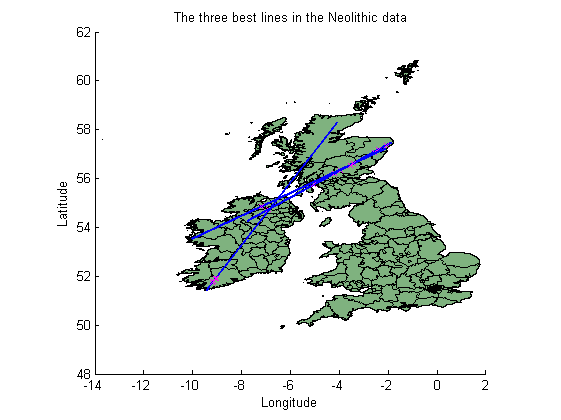
\includegraphics[width=0.5\textwidth]{Best_Line_Sites_3.png}
\caption{\label{fig:Line}The three most densely populated lines in the Neolithic data.}
\end{figure}


\subsection{Results}
When the Hough transform was used on the Neolithic data it was found that most densely populated line had seven points that fell within the tolerance as shown in Figure \ref{fig:Line}, this number alone does not give any information about the significance of the line, so it was necessary to compare this to other data sets. The possibility of these lines occurring by chance had to be taken into consideration before any conclusions could be reached. 
\newline\newline
To test this 1000 sets of uniformly distributed random points were created using the method outlined previously and the most densely populated line in each of these data sets was recorded. From these trials it was found that the maximum number of points within the tolerance was 11, the mean number of points was 5.09 and the standard deviation was 1.88. It can be seen that seven falls just outside one standard deviation of the mean, which initially suggests that seven points is not a significant result. Of the 1000 trials 144 had seven or more points within the tolerance, again as a crude observation this would suggest that the result of seven sites is not significant.
\newline\newline
Figure \ref{fig:Histogram} shows a histogram of the number of points within the tolerance for the random data sets, it can be seen that the data approximately follows a Gaussian distribution with mean 5.09 and standard deviation 1.88. 
\newline\newline
To test whether the result of seven points within the tolerance of the line is statistically significant and unlikely to have occurred by chance a hypothesis test was carried out. The test statistic is the number of points within the tolerance of the most densely populated line, the value of $\alpha$ is set at 5\%, this is the probability of rejecting the null hypothesis when it is true. The null hypothesis was defined as: the data is from a random sample of uniformly distributed data. The alternative hypothesis was defined as: the data is not from a random sample of uniformly distributed data. The test statistic on the Neolithic data set is seven; the probability of a line having seven or more points within the tolerance is 14.4\% from the random trials. This gives a p-value of 0.144 which is greater than $\alpha$, therefore the null hypothesis is accepted which suggests it is likely the value of seven is from a random sample of uniformly distributed data. This strongly suggests that the line in the Neolithic data is a result of chance and is not a significant discovery. Using this method a line needs at least nine points within the tolerance to be considered significant as the probability of finding a line with nine or more points is 1.3\%. This gives a p-value of 0.013 which is less than $\alpha$.  


\begin{figure}[H]
\centering
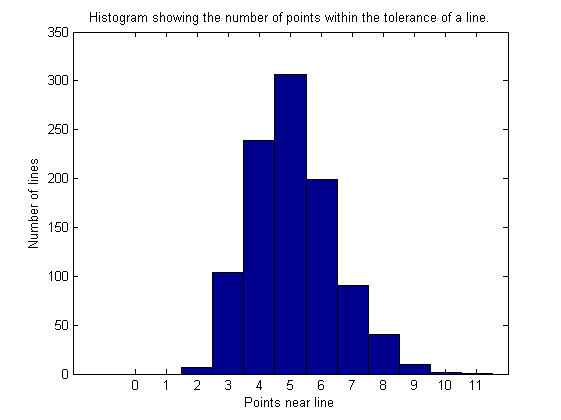
\includegraphics[width=0.5\textwidth]{Histogram_Random_Trial_2.png}
\caption{\label{fig:Histogram}Histogram showing the number of points within the tolerance of the most densely populated line.}
\end{figure}

\section{Clustering The Neolithic Sites}
In addition to the Ley Lines, another pattern that can be looked for in spatial dataset is clusters. A cluster is a group of data points that are deemed near to one another, possibly by being a certain distance from a common point, or being a distance apart that is within a given threshold. A cluster can also be designated as an area of the graph with a higher density of points.
\newline \newline
By looking at the Neolithic sites, it was clear that there were at least 8 densely packed clusters. These are highlighted in Figure \ref{fig:kmeans}. Therefore, it was necessary to find a suitable clustering algorithm which could find these clusters in the Neolithic sites and then be used to find clusters in the random sites.

\begin{figure}[H]
\centering
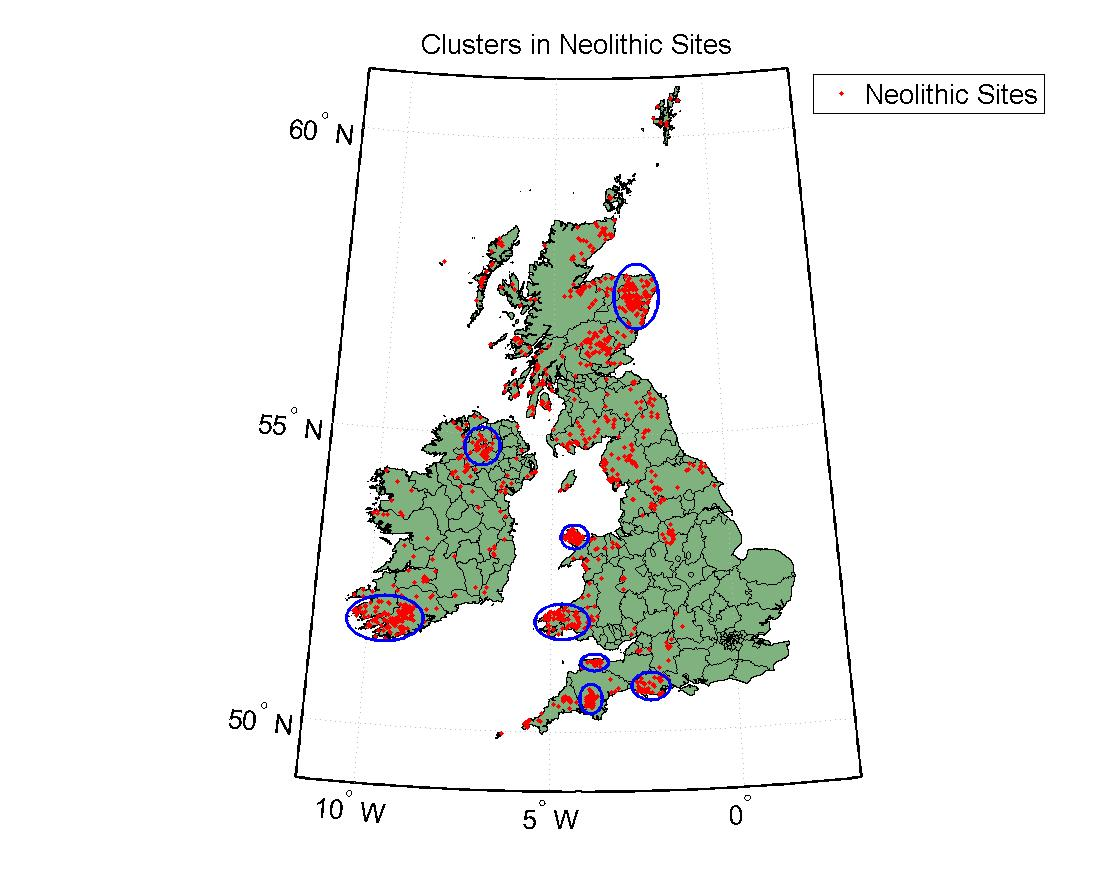
\includegraphics[width=0.5\textwidth]{CNS.jpg}
\caption{\label{fig:CNS}A graph highlighting the 8 most significant clusters in the Neolithic sites.}
\end{figure}

\subsection{Analysis of Different Clustering Algorithms}
There are a variety of algorithms that can be used for determining clusters within datasets, but many of these have limitations that mean they would not be suitable to use with the given data. This is why, although K-Means and Hierarchical Clustering were considered, it was DBSCAN that was used to find the clusters within the Neolithic sites, and also to search for clusters in equally sized sets of random points. 

\subsubsection{K-Means Clustering}
The K-Means Clustering algorithm is one that is commonly used in data analysis. This algorithm works by taking a given number of clusters, and creating a random value, known as the centroid for each. 
\newline\newline
A more accurate centroid is found for each cluster by calculating the distance between that cluster's centroid and each point. The next centroid is taken to be the mean of the points classified to it. The algorithm is then run again with the new centroid. The final centroid is taken to be the point the algorithm converges to. 

\begin{figure}[H]
\centering
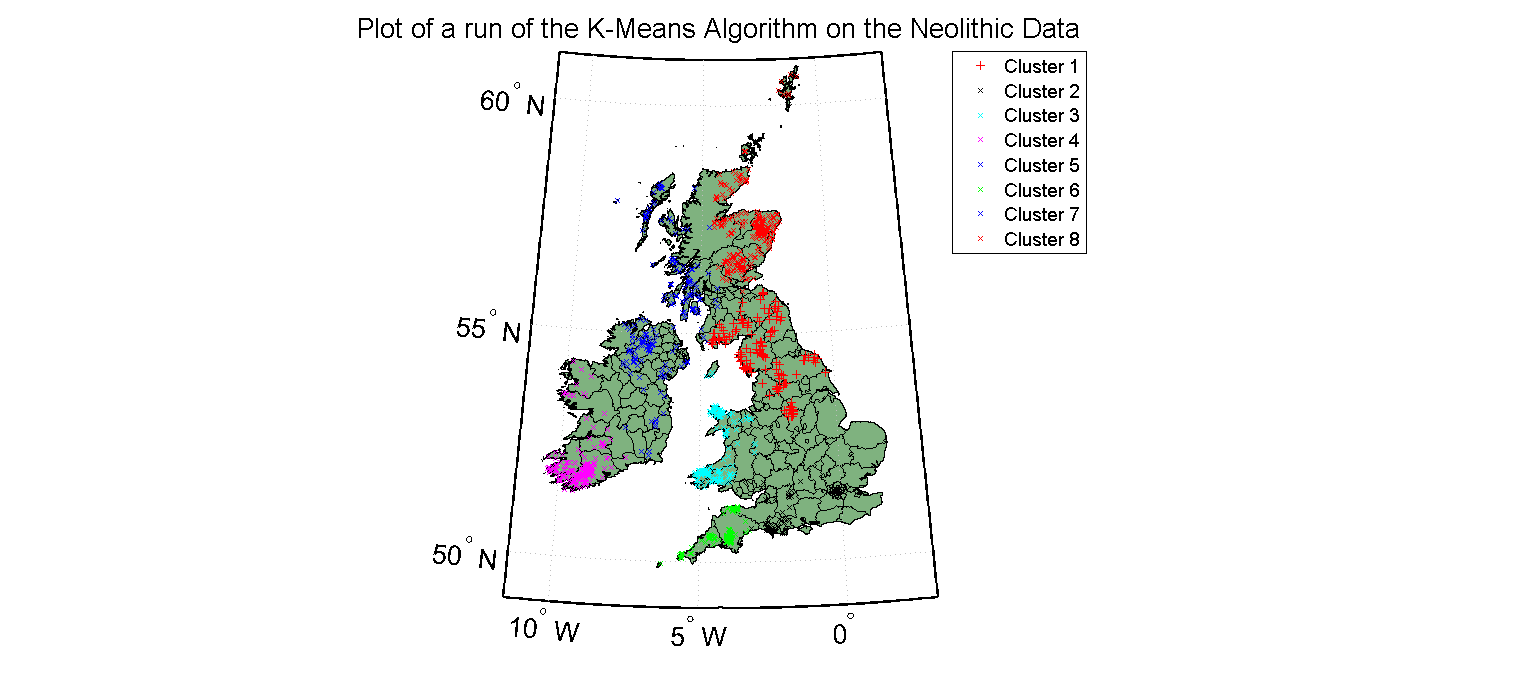
\includegraphics[width=0.8\textwidth]{kmeans.png}
\caption{\label{fig:kmeans}Clusters for the K-Means algorithm.}
\end{figure}
 
This algorithm is not ideal as the number of clusters that the algorithm finds is a variable entered by the user, and not discovered by the algorithm. In the case of the Noelithic sites however it was known that eight clusters existed, so this limitation wasn't much of a hindrance. One of the main issues is that the K-Means algorithm doesn't account for the fact that not every point will certainly belong to a cluster. This can lead to inacurate clusters, with points being clustered that have no correlation with each other, as can be seen in the Midlands in Figure \ref{fig:kmeans}

\begin{figure}[H]
\centering
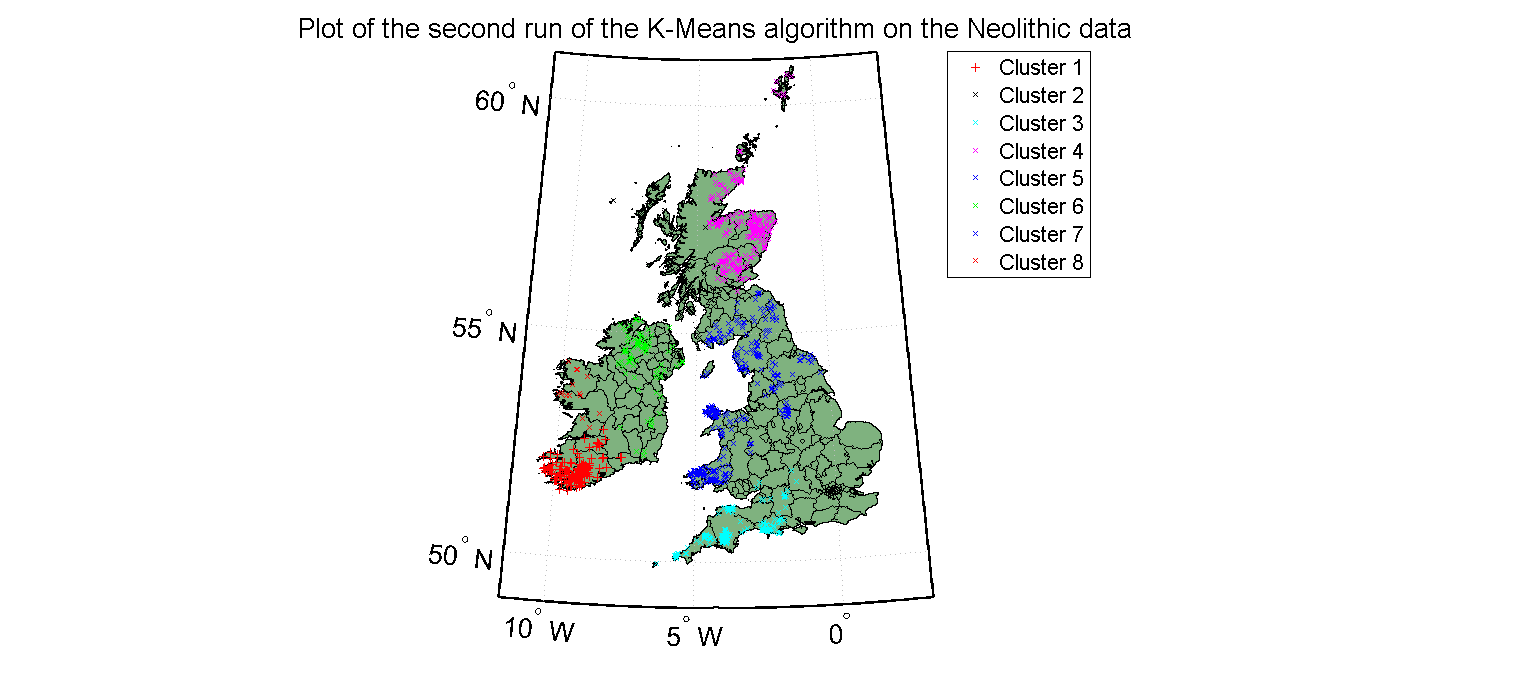
\includegraphics[width=0.8\textwidth]{kmeans2.png}
\caption{\label{fig:kmeans2}Clusters for a second run of the K-Means algorithm.}
\end{figure}

Another issue is the fact that the K-Means algorithm never calculates the same clusters; it always recalculates them. This means that the clusters chosen can be inaccurate, as is shown in the difference between Figure \ref{fig:kmeans2} and Figure \ref{fig:kmeans}. These two limitations mean that K-Means is not a suitable clustering algorithm to use for finding the eight clusters. 

\subsubsection{Hierarchical Clustering}
Hierarchical clustering is a clustering technique that divides a dataset into a sequence of nested partitions \cite{Hierarchical Clustering}. There are two types of hierarchical clustering; divisive and agglomerative. 
\newline\newline
Divisive clustering starts with all the points in a large cluster, and then splits them into smaller clusters, while Agglomerative Clustering starts with each point belonging to a cluster comprising of only themselves, and then joins these clusters together to form larger ones. In order to find the best method for finding the eight clusters, Agglomerative Hierarchical clustering was pursued, as both would find the same result in the end. 
\newline\newline

Agglomerative Hierarchical clustering works by first setting each data point as its own cluster. Then, it calculates the Euclidean distance between each of the points. The algorithm then joins the two points with the lowest distance between them, and joins them in to one cluster. It then repeats, joining clusters together until there is only one singular cluster \cite{matlabagglo}.

\begin{figure}[H]
\centering
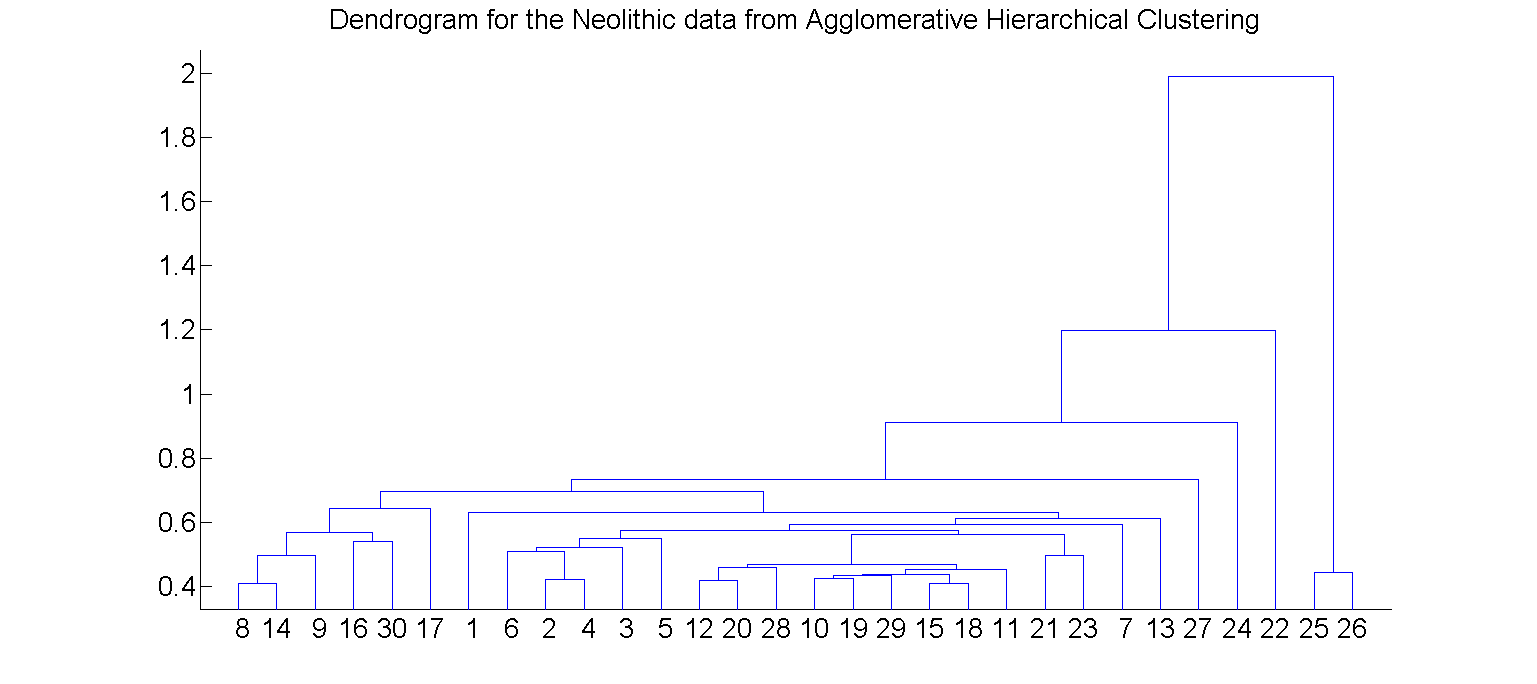
\includegraphics[width=0.8\textwidth]{dendrogram.png}
\caption{\label{fig:dendrogram}Dendrogram created by MATLAB for the neolithic site data. Shows the limitation of MATLAB only showing 30 leaves on the graph.}
\end{figure}

The results from the clustering algorithm can be displayed on a graph in two ways, one by plotting the points as a scatter graph, and the other with a dendrogram\cite{hierarch}. A dendrogram is a tree graph where each of the leaves represents a data point, and where the branches meet represent the different clusters. The manhattan distance between the points is the distance between them when plotted as a scatter graph. 
\newline\newline

\begin{figure}[H]
\centering
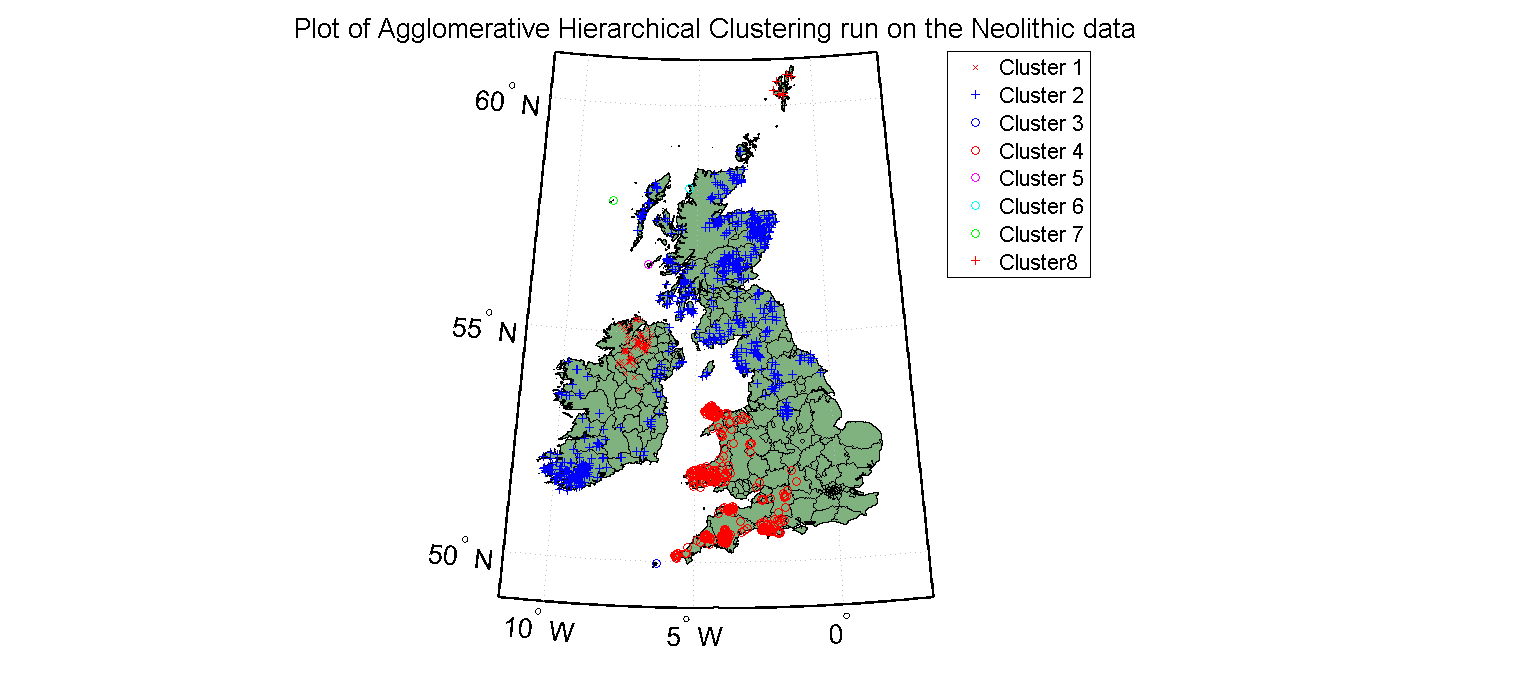
\includegraphics[width=0.8\textwidth]{agglo.png}
\caption{\label{fig:agglo}Plot of all points clustered using Agglomerative Hierarchical Clustering. The large blue cluster shows the inaccuracy.}
\end{figure}

There are a large number of limitations to using Agglomerative Hierarchical clustering, which are the reasons that this method wasn't pursued for the final algorithm. One of these is that the algorithm works by joining points in to clusters, the clusters sometimes seem to be unbelieveable, as can be seen in Figure \ref{fig:agglo}. Here the blue cross cluster stretches across the entirety of the UK, and four clusters are shown as one point. Another limitation is a software-based limitation. The main way to decide where to split the Dendrogram is by using the plot and seeing where the clusters form in the desired way, this is used as a cut off point. The software used to plot the points is MATLAB, and when using this software the Dendrogram function only plots 30 leaves, and it merges other data point leaves together \cite{dendrogram}. This means that calculations of distances between clusters and other information gathering for analysis is made much more difficult. Since there are easier algorithms to use for this task, they were chosen over this.

\subsubsection{DBSCAN}
Density Based Spatial Clustering of Applications with Noise (DBSCAN) is an algorithm that is widely used for clustering spatial data. It works by classifying a minimum number of data points that are densely packed. Any data that is not close enough to a cluster is seen as noise and is subsequently not classified \cite{DBSCAN}. 
\newline \newline
DBSCAN takes three input variables, a set of data points (x), a minimum number of data points needed to form a cluster (k) and a tolerance ($\epsilon$). Every point in the data set has an $\epsilon$-neighbourhood, this is the circular area around a point with the radius $\epsilon$. For a point to belong to a cluster it must have at least one other point within its $\epsilon$-neighbourhood. If the $\epsilon$-neighbourhood of the point contains, at least, the minimum number of points (k) then it is labelled as a core point. If the point belongs to a cluster and has fewer than k points within its $\epsilon$-neighbourhood then it is labelled as a border point. Normally, core points contain significantly more points in their $\epsilon$-neighbourhood than border points. Now, if there is a chain of points from a core point A to a border point B then it is said that point B is density-reachable from point A, however this is not the case vice versa. If there are at least two boarder points within a cluster, then they are said to be density-connected if they do not share a core point but they are both density-reachable from the same core point. A cluster is formed if at least two points are density-reachable or density-connected to each other. Finally, any point that does not belong to any clusters by the of the algorithm is said to be noise and is not classified \cite{DBSCAN}. 
\newline \newline
One advantage of DBSCAN is that it does not classify every data point. This means that only the data within the significant clusters can be analysed while the remaining data points can be disregarded. Another advantage of DBSCAN is that, unlike k-means, it does not ask for a given number of clusters to be searched for. This means that data points will not be forced into a cluster that they clearly do not belong to. Because of these two advantages the DCSCAN algorithm could be used to easily find different sized clusters in the Neolithic sites. 
\newline \newline
The DCSCAN algorithm (provided by The University of Silesia \cite{DBSCANfunc}) was tested by trying to find the 8 clusters highlighted in Figure \ref{fig:CNS}. They were all easily found when the parameters k=30 and $\epsilon$=0.2 were used, as shown in Figure \ref{fig:CDB}.

\begin{figure}[H]
\centering
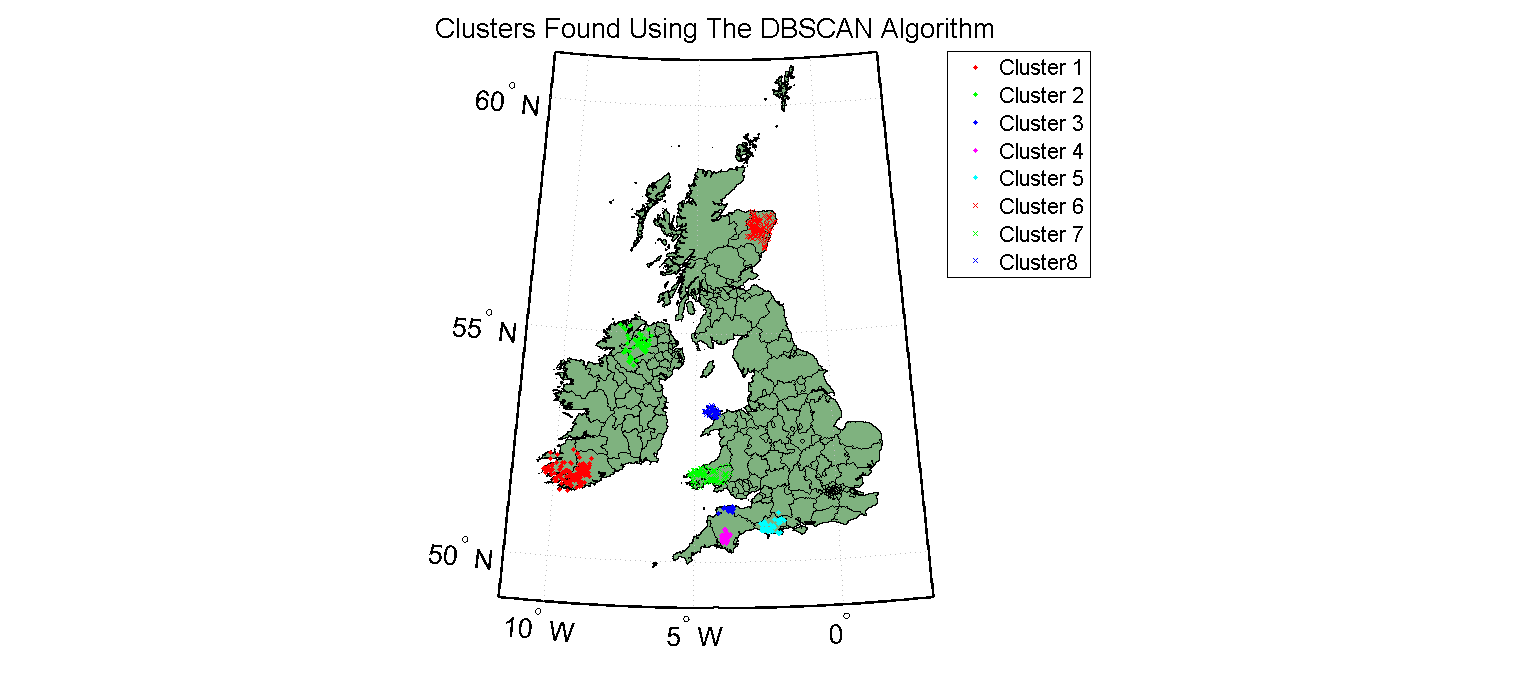
\includegraphics[width=0.8\textwidth]{CDB.png}
\caption{\label{fig:CDB} A graph showing 8 clusters which have been found using the parameters k=30 and $\epsilon$=0.2 in the DBSCAN algorithm. These clusters are exactly the same as those highlighted in Figure \ref{fig:CNS}. This suggests that DBSCAN algorithm is the preferable method.}
\end{figure}

Because of the way the DBSCAN algorithm works, and the parameter inputs needed, it was clear that this algorithm would work better than both the k-mean algorithm and the hierarchical clustering when searching for an unknown number of clusters in the random sites so, this was the algorithm of choice. 

\subsection{Finding Clusters In Random Sites}
To find clusters in the random sites it was necessary to find a range of parameters to use in the DBSCAN algorithm. These had to range in strictness, from parameters that would find the large and dense clusters in the random sites to parameters which would look for much smaller and less dense clusters. To start with, the largest and most dense cluster in the Neolithic sites was found. This is shown in Figure \ref{fig:LMDC}. 

\begin{figure}[H]
\centering
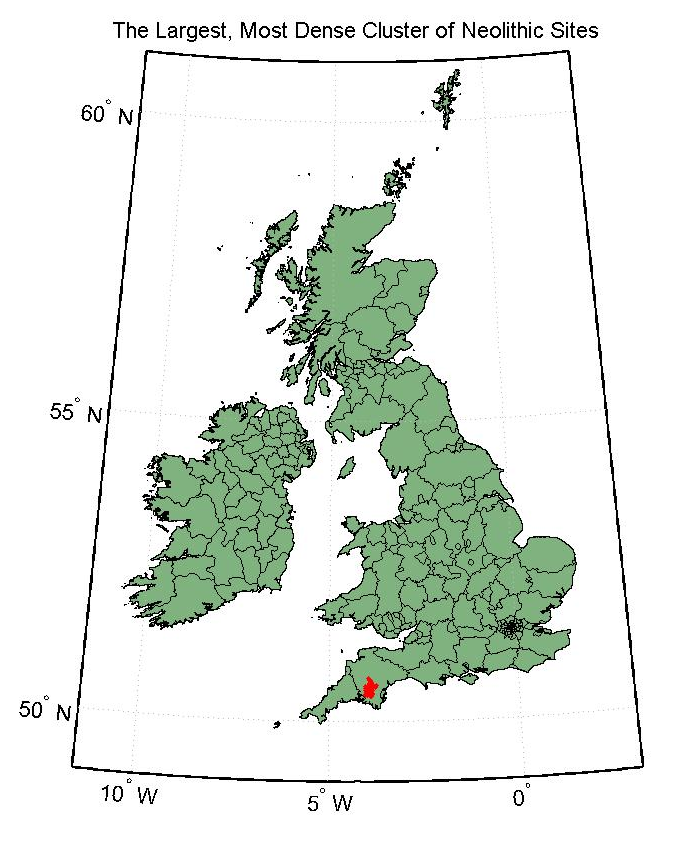
\includegraphics[width=0.35\textwidth]{LMDC.png}
\caption{\label{fig:LMDC} A graph showing the largest and most dense cluster in the Neolithic sites. This is found when using the parameters k=113 and $\epsilon$=0.18 in the DBSCAN algorithm.}
\end{figure}

The same parameters used to find this cluster (k=113 and $\epsilon$=0.18) were then used to try and find the clusters in the random sites, which were at least the same size as the largest cluster of Neolithic sites. The next pair of parameter used were the parameters which found the 8 clusters in Figure \ref{fig:CDB} (k=30 and $\epsilon$=0.2). This allowed reasonably, yet still significantly, sized clusters to be found in the random sites. Finally, a lenient pair of parameters (k=20 and $\epsilon$=0.25) were used. As Figure \ref{fig:LCNS} shows, these parameters find some questionable clusters (e.g Cluster 9) in the Neolithic sites, however some of the clusters (e.g Cluster 5) were reasonable. This allowed some less dense clusters to be found in the random sites. 

\begin{figure}[H]
\centering
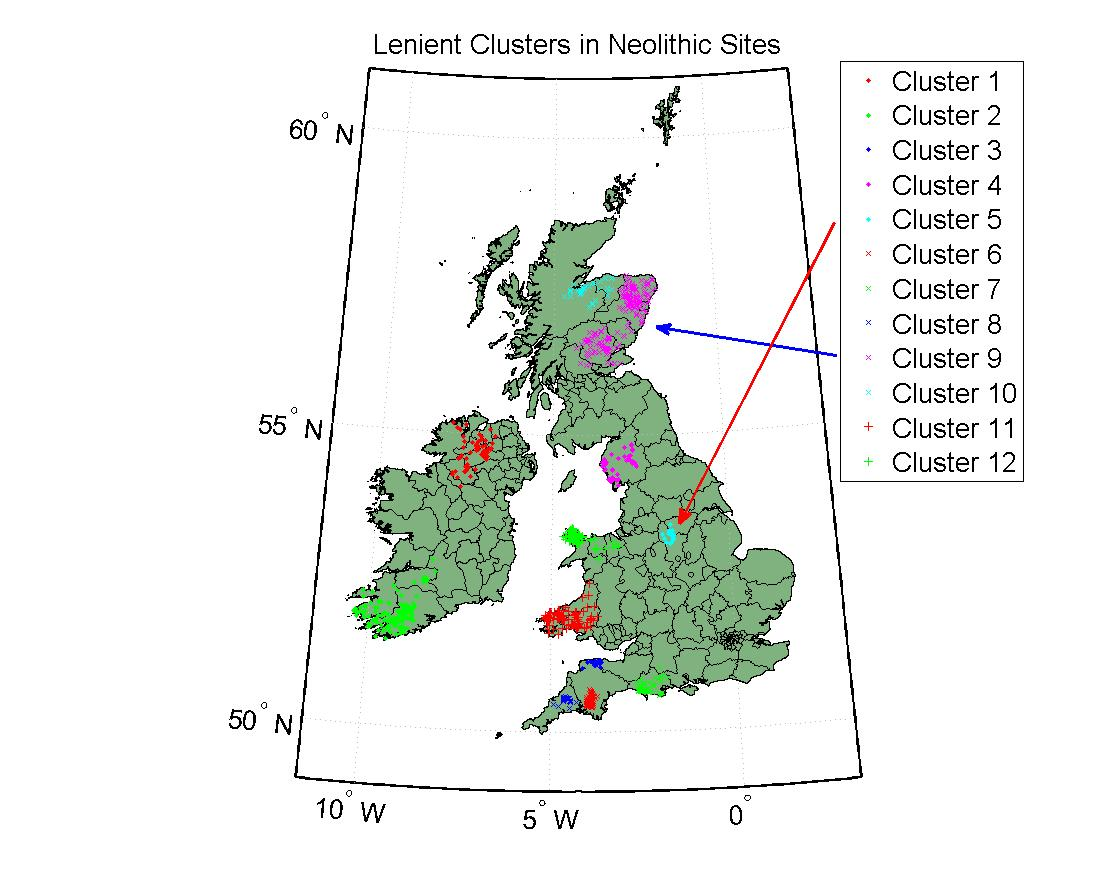
\includegraphics[width=0.5\textwidth]{LCNSv2.jpg}
\caption{\label{fig:LCNS}A graph showing 12 clusters of Neolithic sites. These were produced by using the parameters k=20 and $\epsilon$=0.25 in the DBSCAN algorithm.}
\end{figure}

For each of the three pairs of parameters stated above, clusters were searched for in 1000 different sets of random sites. All of the coordinates for the random sites and the number of clusters found in each set were recorded. This was so any clusters found could be analysed further.

\subsection{Results}
To find the significance of the clusters in the Neolithic sites, hypothesis testing was used on each of the 3 pairs of parameters stated above. For each of the tests, the test statistic was defined as the number of clusters produced by the DBSCAN algorithm for the two parameters k and $\epsilon$. A null hypothesis for each test was created stating that, for the given parameters, any clusters found in the Neolithic sites could be found in the uniformly distributed random sites. An alternative hypothesis for each test was also created. This stated that the clusters found in Neolithic sites could not be found in the random sites. The significance level ($\alpha$) for each test was 5\%.
\newline \newline
For the first test, the parameters k=113 and $\epsilon$=0.18 were used to find the largest and most dense clusters in the Neolithic sites. This meant that the test statistic was 1. Clusters with the same parameters were then looked for in 1000 sets of random sites. Not a single cluster was found which infers that there is a p-value of less than 0.001. This p-value is much lower than the significance level (0.05), which means that the null hypothesis can be rejected and the alternative hypothesis can be accepted. This implies that the largest and most dense cluster in the Neolithic sites did not occur by chance.
\newline \newline
For the second test, the parameters k=30 and $\epsilon$=0.2 were used to find the 8 most prolific clusters in the Neolithic sites. This meant that the test statistic was 8. Once again, no clusters were found in 1000 sets of random sites, which means that there is a p-value of less than 0.001. This p-value is much lower than the significance level (0.05) which means that the null hypothesis can be rejected and the alternative hypothesis is accepted. This implies that the 8 largest and most significant clusters in the Neolithic sites did not occur by chance.
\newline \newline
For the final test, 12 clusters were found in the Neolithic sites using the parameters k=20 and $\epsilon$=0.25. This meant that the test statistic was 12. Using these parameters, 1 cluster was found in five of the one thousand tests. However, on closer inspection of the clusters found, it could be seen that the random sites had been incorrectly clustered, as illustrated in Figure \ref{fig:ICRS}. This is because the parameters used were too lenient. 

\begin{figure}[H]
\centering
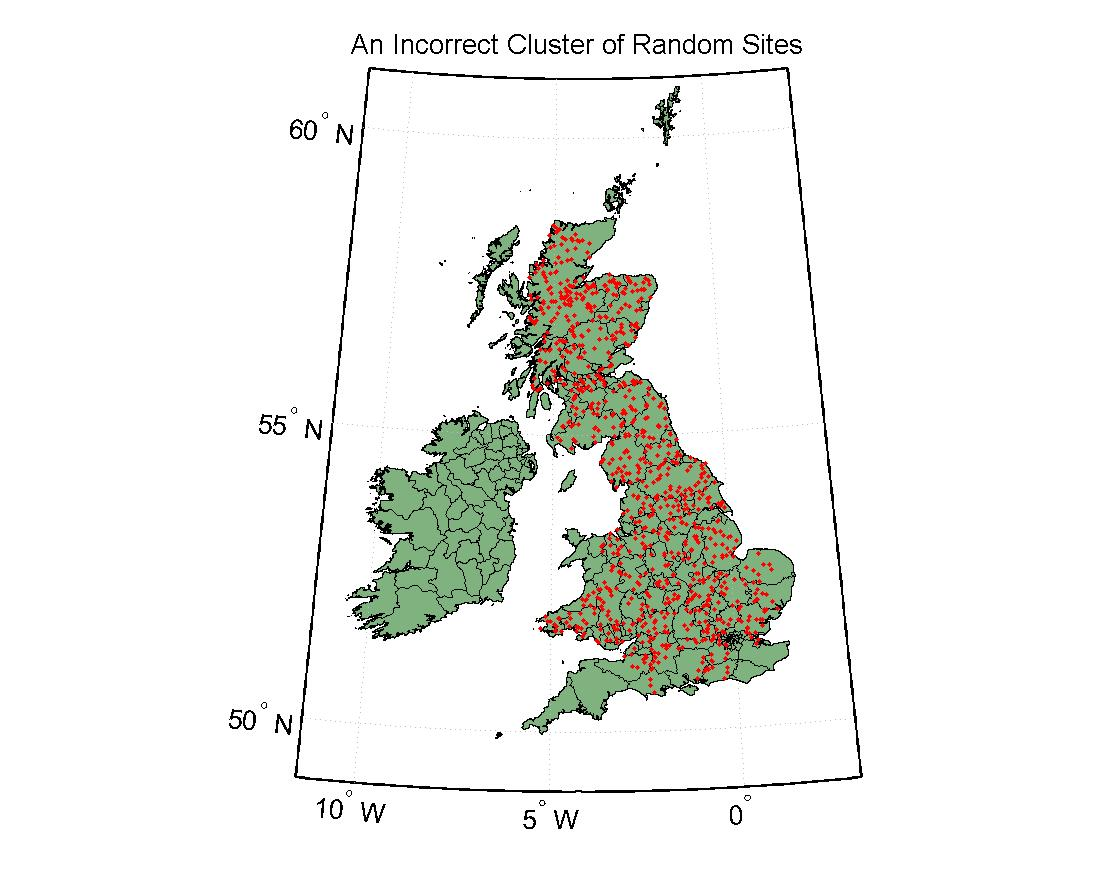
\includegraphics[width=0.5\textwidth]{ICRS.jpg}
\caption{\label{fig:ICRS}A graph showing one of the "clusters" found in the random sites when the parameters k=20 and $\epsilon$=0.25 were used in the DBSCAN algorithm. This is clearly not a true cluster and was produced because the k and $\epsilon$ parameters were too lenient.}
\end{figure}

Since all five of the clusters found were incorrect, once again the p-value was less than 0.001. This means that the null hypothesis can be rejected and the alternative hypothesis is accepted, implying that all of the significant clusters found in the Neolithic sites do not occur by chance. 

\section{Analysis of Results}
This investigation set out to determine whether there are any significant linear patterns in the location of Neolithic sites. It has shown that alignments exist however there is a high probability that they occurred by chance and are not statistically significant. This provides significant evidence against the theory that these lines were created to serve a purpose in Neolithic times. While no significant patterns were observed in the alignments a strong pattern was found in the clustering. This pattern was not observed in the random data so is unlikely to have occurred by chance. This is a significant result and could have many possible explanations; one interpretation links the sites to nutrient-rich river valleys \cite{explanation}.  
\newline\newline
It was theorised that one reason for the lack of Ley Lines found in the data may be the growth of civilisation across the country. It was suggested that many Neolithic sites were destroyed by later civilisations as they built their own settlements. The lack of Neolithic sites in London and the South East is particularly notable, and it may be possible that the constant modernisation and expanse of London has led to the building over and destruction of many ancient or historic sites. 
\newline\newline
To research further, collecting the locations of notable sites throughout further periods of history could lead to the discovery of statistically relevant lines linking them. One particular subject for this study could be churches, as many of the Ley Lines that people claim to have found take religious sites as their points. An interesting extension to the project could be finding the validity of "known" Ley Lines, such as the St Michael's Ley Line, and investigating the number of different period's sites which had to be added to the data to find the existence of this line.
 
\pagebreak
\begin{thebibliography}{1}

\bibitem{Alfred Watkins}Watkins, A (1921). {\em The Old Straight Track}. London: Simkin, Marshall, Hamilton and Kent. p9-11.

\bibitem{GAA} Global Administrative Areas, \url{http://www.gadm.org/}, [Viewed 04/04/2014].

\bibitem{Hough Transform} Amos Storkey (2000). {\em Hough Transform.}  \url{ http://homepages.inf.ed.ac.uk/amos/hough.html} [viewed 03/04/2014].

\bibitem{Hough Transform 2} The Indian Institute of Technology Madras (2009). {\em Hough Transform.} \url{ http://www.cse.iitm.ac.in/~sdas/vplab/courses/CV_DIP/PDF/LECT_smooth_HT.pdf} [Viewed 03/04/2014].

\bibitem{Hierarchical Clustering} Gan, G, Ma, C, Wu, J (2007). {\em Data Clustering Theory, Algorithms, and Applications}. p109-149.

\bibitem{hierarch} (2008).{\em Hierarchical Agglomerative Clustering} \url{http://nlp.stanford.edu/IR-book/html/htmledition/hierarchical-agglomerative-clustering-1.html} [Viewed 23/03/2014]

\bibitem{dendrogram} MathWorks (2014). {\em Dendrogram plot}. \url{http://www.mathworks.co.uk/help/stats/dendrogram.html} [Viewed 03/04/2014].

\bibitem{matlabagglo} EE-Programmer (2011). {\em MATLAB Tutorial - k-means and hierarchical clustering}. \url{http://www.eeprogrammer.com/tutorials/Matlab/cluster.html} 
[Viewed 19/03/2014].

\bibitem{DBSCAN} Hendrik B{\"a}cklund et al (2011), `DBSCAN', {\em A Density-Based Spatial Clustering of Application with Noise},  \url{http://staffwww.itn.liu.se/~aidvi/courses/06/dm/Seminars2011/DBSCAN(4).pdf} [Viewed 26/03/2014].

\bibitem{DBSCANfunc} Michal Daszykowski (2004), DBSCAN Matlab function, url{http://chemometria.us.edu.pl/download/DBSCAN.M}, [viewed 04/04/2014].

\bibitem{explanation} Sergei Fedotov. (2013), {\em The growth of human settlements during the Neolithic, clustering and food crisis.} \url{http://arxiv.org/pdf/0804.3060v1.pdf.} [Viewed  04/04/2013].

\end{thebibliography}

\end{document}